\section{Adversary Simulation}

\noindent This section presents a simulated contest between a social networking website publishing neighborhoods and an adversary looking to determine existing edges from these neighborhoods. The website, knowing the original social network, uses the label-swapping algorithm multiple times and tracks the frequency each edge appears (edges that never occur in an output of label-swapping are ignored). For some $\epsilon,\delta \in [0,1]$, test the proportion of edges that occur with a frequency in $[0.5-\delta,0.5+\delta]$. If that proportion is less than $\epsilon$, increment $k$ and repeat the process. If $k$ reaches some set maximum (say 6), stop the process: k has become too large for the k-neighborhoods to hold any meaningful information. If the proportion is greater than $\epsilon$, set $k' = k$.  Figure \ref{k_vals} shows the determined k' values for various $\mu$ values. We belive that $k'$ is the minimum $k$ value to sufficiently disguise the given graph. \\

\indent To test this theory, we pass the k'-neighborhood of $G$ to the edge-adding algorithm and attempt to reconstruct $G$. The sucess of this attempt is measured by the proportion of edges the algorithm yields that are in $G$.\\

\begin{figure}[H]
  \label{k_vals}
\centerline{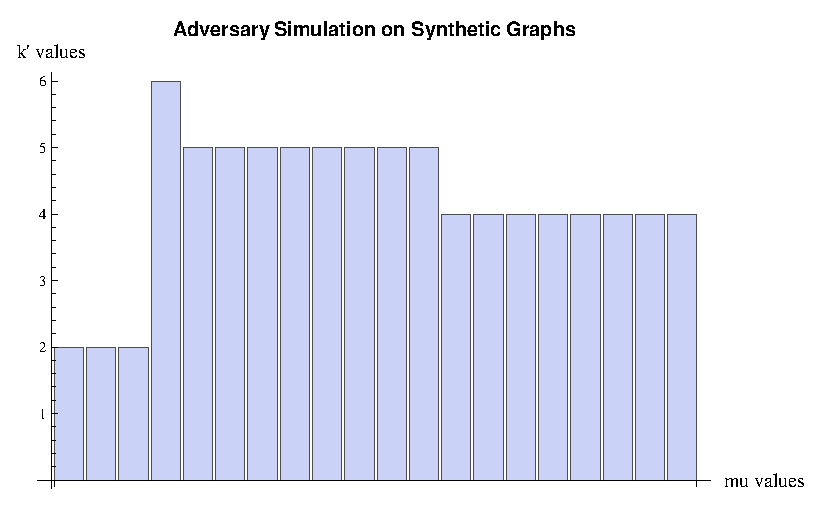
\includegraphics[scale=0.3]{k_values.eps}}
  \caption{Returned k' values for synthetic graphs of different mu values.}
  \label{fig:k'_values}
\end{figure}
